\documentclass[10pt,a4paper]{article}

\usepackage[latin1]{inputenc}
\usepackage{amsmath}
\usepackage{amsfonts}
\usepackage{amssymb}
\usepackage{graphicx}
\usepackage{listings}
\title{Assignment No :B9}
\date{}
\author{Roll No.4431}


\begin{document}
\maketitle
\section{Title:}
BAI tool for shopping mall.

\section{Problem Definition}
A Mall has number of items for sale. Build a required Database to develop BAI tool for considering one aspect of growth to the business Such as organization of products based on demand and patterns use R Programming or other equivalent latest tools used in Industry.


\section{Learning Objectives}
\begin{enumerate}
\item To understand the concept of Business Analytics and Intelligence.
\item To identify BAI opportunities in real world businesses.
\end{enumerate}

\section{Learning Outcomes}
\begin{enumerate}
\item Ability to apply BAI tools to real world business problems.
\item Acquire proficiency over BAI and its theoretical aspects by applying them in practical.
\end{enumerate}


\section{Related Mathematics}

{\rmfamily
	mathematical model is given as below,}


\bigskip

\textrm{S=X,Y,Mem-shared,DD,NDD,Fme,D,Dsupp,conf,lk,ck,subset(),apriori-gen(),rules}


\bigskip

{\rmfamily
	Where,}

{\rmfamily
	X=input
	Datasets of Groceries.
	}

{\rmfamily
	Supp= frequency count of itemset in D dataset
	support=support(A+B)/N
	}

{\rmfamily
	support=support(A+B)/N
}

{\rmfamily
	conf=support(A+B)/support(A)
	
{\rmfamily
lk=large item set.	
	}
	
	{\rmfamily
		ck=set of k itemset
	}
	
	{\rmfamily
Y=output
Bar chart of frequency distribution of grocery items.

	{\rmfamily
	
 Rules:Association rules
 
}
{\rmfamily
		Mem-shared=memory shared by the applications.}
	
{\rmfamily
		DD=Deterministic Data
		Grocery data.
}
	
	{\rmfamily
NDD=Non-Deterministic Data.}

{\rmfamily
Fme= subset()
To check whether subsets are large item sets or not
}

\section{Concepts related theory}
\subsection{Algorithm used (Apriori) : }

  1.Find all itemsets with a specified minimal support  (coverage ).
\newline 
An itemset is just a specific set of items, e.g. {apples, cheese}. The Apriori algorithm can efficiently find all itemsets whose coverage is above a given minimum.

2.Use these itemsets to help generate interersting rules.
\newline
Having done stage 1, we have considerably narrowed down the possibilities, and can do reasonably fast processing of the large itemsets to generate candidate rules

Find all large 1-itemsets
\newline
2:  For (k = 2 ; while Lk-1 is non-empty; k++)
\newline
3		{Ck = apriori-gen(Lk-1)
\newline	
4          For each c in Ck, initialise c.count to zero 
\newline
5          For all records r in the DB
	{Cr = subset(Ck, r);  For each c in Cr , c.count++ }
\newline	
	7             Set Lk := all c in Ck whose count >=  minsup
\newline
	8         }  /*  end   -- return all of the Lk sets.

R programming Introduction:
\newline
It is common for today's scientific and business industries to collect large amounts of data, and the ability to
analyze the data and learn from it is critical to making informed decisions. Familiarity with software such as R
allows users to visualize data, run statistical tests, and apply machine learning algorithms. Even if you already
know other software, there are still good reasons to learn R:
\newline
1.	 R is free. If your future employer does not already have R installed, you can always download it for free,
unlike other proprietary software packages that require expensive licenses. No matter where you travel, you
can have access to R on your computer.
\newline
2.	 R gives you access to cutting-edge technology. Top researchers develop statistical learning methods
in R, and new algorithms are constantly added to the list of packages you can download.
\newline
3.	 R is a useful skill. Employers that value analytics recognize R as useful and important. If for no other
reason, learning R is worthwhile to help boost your resume.
\newline
Note that R is a programming language, and there is no intuitive graphical user interface with buttons you can
\newline
click to run different methods. However, with some practice, this kind of environment makes it easy to quickly
code scripts and functions for various statistical purposes. To get the most out of this tutorial, follow the examples
by typing them out in R on your own computer. A line that begins with > is input at the command prompt. We
do not include the output in most cases, but you should try out the commands yourself and see what happens.
If you type something at the command line and decide not to execute, press the down arrow to clear the line;
pressing the up arrow gives you the previous executed command.

\section{Algorithm : }

Apriori Algorithm:
\newline
1.Find all itemsets with a specified minimal support  (coverage ).  An itemset is just a specific set of items, e.g. {apples, cheese}. The Apriori algorithm can efficiently find all itemsets whose coverage is above a given minimum.2.Use these itemsets to help generate interersting rules. Having done stage 1, we have considerably narrowed down the possibilities, and can do reasonably fast processing of the large itemsets to generate candidate rules


:  Find all large 1-itemsets
\newline
2:  For (k = 2 ; while Lk-1 is non-empty; k++)
\newline

3		{Ck = apriori-gen(Lk-1)
\newline

	4          For each c in Ck, initialise c.count to zero 
\newline

	5          For all records r in the DB
	{Cr = subset(Ck, r);  For each c in Cr , c.count++ }
\newline

	7             Set Lk := all c in Ck whose count >=  minsup
\newline

	8         }  /*  end   -- return all of the Lk sets.


\begin{center}
	\begin{figure}[!htbp]
		\centering
		\fbox{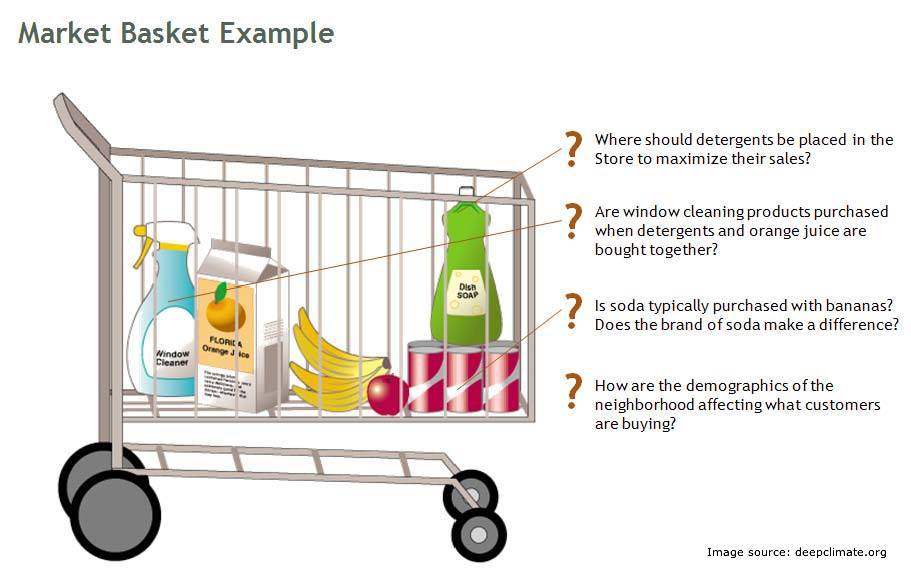
\includegraphics[width=\textwidth]{association.png}}
		\caption{association rule}
		\label{fig:usecase}
	\end{figure}
\end{center}  

the following association rules: (Rules are just for illustrations and understanding of the concept. They might not represent the actuals).
\newline
Rule 1: If Milk is purchased, Then Sugar is also purchased.
\newline
Rule 2:  If Sugar is purchased, Then Milk is also purchased.
\newline
Rule 3: If Milk and Sugar is Purchased, Then Coffee powder is also purchased in 60percent of the transactions.
\newline
Generally association rules are written in "IF-THEN" format. We can also use the term "antecedent" for IF and "Consequent" for THEN.


From the above rules, we understand the following explicitly:
\newline
1.	Whenever Milk is purchased, Sugar is also purchased or vice versa. 
\newline
2.	If Milk and Sugar is purchased then coffee powder is also purchased. This is true in 3 out of the 5 transactions. In other words we can say that we have a support of 3 out of 5 transactions for this rule. (60percent possibility). 

\begin{itemize}
\item Frequent item set :- Item set occurring in high frequency. For example in our Coffee dataset, Milk and sugar combinations occurred in 100percent of the transactions.
\item Support:-  The support for the rule indicates its impact in terms of overall size.  If only a small number of transactions are affected, the rule may be little use. For example, the support of "IF Milk and Sugar THEN Coffee powder" is 3/5 transactions or 60percent of the total transactions.
\item Confidence :- It determines the operational usefulness of a rule. Transactions with confidence with more than 50percent will be selected.  For example, the confidence of milk, sugar and coffee powder given milk, coffee can be written as
Number of transactions that include Milk and Sugar (Antecedent) and Coffee Powder (Consequent) is 3
Number of transactions that contains only Milk and Sugar (Antecedent)) is 5.
\newline
P(Milk and Sugar AND Coffee Powder)/ P (Milk and Sugar)  =  3/5 = 60percent

\end{itemize}

\section{Output}
Output :
R program Introduction:
R version 3.0.2 (2013-09-25) -- "Frisbee Sailing"
\newline
Copyright (C) 2013 The R Foundation for Statistical Computing
Platform: x86 - 64-pc-linux-gnu (64-bit) R is free software and comes 
with ABSOLUTELY NO WARRANTY. You are welcome to redistribute it under certain conditions. Type 'license()' or 'licence()' for distribution details. Natural language support but running in an English localeR is a collaborative project with many contributors. Type 'contributors()' for more information and 'citation()' on how to cite R or R packages in publications.Type 'demo()' for some demos, 'help()' for on-line help, or'help.start()' for an HTML browser interface to help. Type 'q()' to quit R.
\newline
: 2+2
\newline
[1] 4
\newline
: 3+4
\newline
[1] 7
\newline
: 3/5
\newline
[1] 0.6
\newline
: log(100,base=10)
\newline
[1] 2
\newline
: exp(12)
\newline
[1] 162754.8
\newline
: runif(10)
\newline
[1] 0.33166502 0.22091722 0.28724449 0.61601346 0.13121878 0.27327015
\newline
[7] 0.22955652 0.09091556 0.04072079 0.05192992
\newline
: runif(2)
[1] 0.2017608 0.1082742
\newline
: plot(runif(10))
\newline
: x<-runif(15)
\newline
: plot(x)
\newline
: x[4]
[1] 0.492467
\newline
: plot(x[4])
\newline
: x<-2+2
\newline
: y<-3+3
\newline
: s<-"Hello"
\newline
: s
[1] "Hello"
\newline
: y
[1] 6
\newline
: x
[1] 4
\newline
: v<-c(2,3,4,5)
\newline
: v
[1] 2 3 4 5
\newline
: v1<-seq(0,1,length=11)
\newline

: v1
[1] 0.0 0.1 0.2 0.3 0.4 0.5 0.6 0.7 0.8 0.9 1.0
\newline
: v1<-seq(1,10,length=11)
\newline
: v1
\newline
[1]  1.0  1.9  2.8  3.7  4.6  5.5  6.4  7.3  8.2  9.1 10.0
\newline
: v1<-seq(1,100,length=100)
\newline
: v1
\newline
[1]   1   2   3   4   5   6   7   8   9  10  11  12  13  14  15  16  \newline
17  18
\newline
[19]  19  20  21  22  23  24  25  26  27  28  29  30  31  32  33  34  \newline
35  36
\newline
[37]  37  38  39  40  41  42  43  44  45  46  47  48  49  50  51  52  \newline
53  54
\newline
[55]  55  56  57  58  59  60  61  62  63  64  65  66  67  68  69  70  \newline
71  72
\newline
[73]  73  74  75  76  77  78  79  80  81  82  83  84  85  86  87  88  \newline
89  90
\newline
[91]  91  92  93  94  95  96  97  98  99 100
\newline
: 1:10
\newline
[1]  1  2  3  4  5  6  7  8  9 10
\newline
: v<-height/weight
\newline
Error: object 'height' not found
\newline
: v<-height
\newline
Error: object 'height' not found
\newline
: v<-height=1
\newline
Error in (v <- height) = 1 : could not find function "<-<-"
\newline
: v<-v1/v2
\newline
Error: object 'v2' not found
\newline
: sum(v)
\newline
[1] 14
\newline
: length(v)
\newline
[1] 4
\newline
: w<-mean(v)
\newline
: w
\newline
[1] 3.5
\newline
: a<-median(v)
\newline
: a
\newline
[1] 3.5
\newline
: sd(v)
\newline
[1] 1.290994
\newline
: var(v)
\newline
[1] 1.666667
\newline
: IQR(v)
\newline
[1] 1.5
\newline
: fivenum(v)
\newline
[1] 2.0 2.5 3.5 4.5 5.0
\newline
: summery(v)
\newline
Error: could not find function "summery"
\newline
: summary(v)
\newline
\begin{table}[!htbp]
	\begin{center}
		\def\arraystretch{2.0}
		\begin{tabular}{| p{2cm} | p{2cm} | p{2cm} | p{2cm} | p{2cm} | p{2cm}}
			\hline
			Min.	& 1st Qu.	& Median	& Mean	& 3rd Qu. & Max \\
			\hline
			2.00 & 2.75 & 3.50 & 3.50 & 4.25 & 5.00
			\\
			\hline
			
		\end{tabular}
	
		\label{tab:hreq}
	\end{center}	
\end{table}


: v1<-c(1,2,3,4)
\newline
: v2<-c(5,6,7,8)
\newline
: cbind(v1,v2)
\newline
v1 v2
\newline
[1,]  1  5
\newline
[2,]  2  6
\newline
[3,]  3  7
\newline
[4,]  4  8
\newline
: rbind(v1,v2)
\newline
[,1] [,2] [,3] [,4]
\newline
v1    1    2    3    4
\newline
v2    5    6    7    8
\newline
: v<-seq(from=1,to=10,by=1)
\newline
: matrix(v,nrow=3,ncol=4)
\newline

     [,1] [,2] [,3] [,4]
\newline
     
     [1,]    1    4    7   10
\newline

     [2,]    2    5    8    1
\newline
    
     [3,]    3    6    9    2
\newline

: matrix(v,nrow=3,ncol=4, byrow=TRUE)
\newline
[,1] [,2] [,3] [,4]
\newline

[1,]    1    2    3    4
\newline

[2,]    5    6    7    8
\newline

[3,]    9   10    1    2
\newline
: v<-seq(from=1,to=20,by=1)
\newline
: m1<-matrix(v,nrow=3,ncol=4)
\newline
: m1
\newline
[,1] [,2] [,3] [,4]
\newline
[1,]    1    4    7   10
\newline
[2,]    2    5    8   11
\newline
[3,]    3    6    9   12
\newline
: colnames(m1)<-c("c1","c2","c3","c4")
\newline
: rownames(m1)<-c("row1","row2","row3")
\newline
: m1
\newline
c1 c2 c3 c4
\newline
row1  1  4  7 10
\newline
row2  2  5  8 11
\newline
row3  3  6  9 12
\newline
: m1[,]
\newline
c1 c2 c3 c4
\newline
row1  1  4  7 10
\newline
row2  2  5  8 11
\newline
row3  3  6  9 12
\newline
: m1[,"c2"]
\newline
row1 row2 row3 
\newline
4    5    6 
\newline
: m1[,2]
\newline
row1 row2 row3 
\newline
4    5    6 
\newline
: m1[2,4]
\newline
[1] 11
\newline
: length(v)
\newline
[1] 20
\newline
: nrow(m1)
\newline
[1] 3
\newline
: ncol(m1)
\newline
[1] 4
\newline
: : data(Bfox)
\newline
: Bfox
\newline
partic  tfr menwage womwage   debt parttime
\newline
1946   25.3 3748   25.35   14.05  18.18    10.28
\newline
1947   24.4 3996   26.14   14.61  28.33     9.28
\newline
1948   24.2 3725   25.11   14.23  30.55     9.51
\newline
1949   24.2 3750   25.45   14.61  35.81     8.87
\newline
1950   23.7 3669   26.79   15.26  38.39     8.54
\newline
1951   24.2 3682   26.33   14.58  26.52     8.84
\newline
1952   24.1 3845   27.89   15.66  45.65     8.60
\newline
1953   23.8 3905   29.15   16.30  52.99     5.49
\newline
1954   23.6 4047   29.52   16.57  54.84     6.67
\newline
1955   24.3 4043   32.05   17.99  65.53     6.25
\newline
1956   25.1 4092   32.98   18.33  72.56     6.32
\newline
1957   26.2 4168   32.25   17.64  69.49     7.30
\newline
1958   26.6 4073   32.52   18.16  71.71     8.65
\newline
1959   26.9 4100   33.95   18.58  78.89     8.80
\newline
1960   27.9 4119   34.63   18.95  84.99     9.39
\newline
1961   29.1 4159   35.14   18.78  87.71    10.23
\newline
1962   29.9 4134   34.49   18.74  95.31    10.77
\newline
1963   29.8 4017   35.99   19.71 104.40    10.84
\newline
1964   30.9 3886   36.68   20.06 116.80    11.70
\newline
1965   32.1 3467   37.96   20.94 130.99    12.33
\newline
1966   33.2 3150   38.68   21.20 135.25    12.18
\newline
1967   34.5 2879   39.65   21.95 142.93    13.67
\newline
1968   35.1 2681   41.20   22.68 155.47    13.82
\newline
1969   36.1 2563   42.44   23.75 165.04    14.91
\newline
1970   36.9 2571   42.02   25.63 164.53    15.52
\newline
1971   37.0 2503   45.32   26.79 169.63    15.47
\newline
1972   37.9 2302   45.61   27.51 190.62    15.85
\newline
1973   40.1 2931   45.59   27.35 209.60    15.40
\newline
1974   40.6 1875   48.06   29.64 216.66    16.23
\newline
1975   42.2 1866   46.12   29.33 224.34    16.71: 
\newline

:dataset<-read.csv("/home/pccoe/Desktop/IRIS.csv")
\newline




Program:
\newline
* Shopping Mall Market Basket Analysis for Grocery data set 
\newline

* Load the libraries
\newline
library(arules)
\newline
library(arulesViz)
\newline
library(datasets)
\newline

* Load the data set
\newline
data(Groceries)
\newline

* show Groceries data set details
\newline
Groceries
\newline

* Create an item frequency plot for the top 20 items
\newline
itemFrequencyPlot(Groceries,topN=20,type="absolute")
\newline

* Get the rules
\newline
rules <- apriori(Groceries, parameter = list(supp = 0.001, conf = 0.8))
\newline

* Show the top 5 rules, but only 2 digits
\newline
options(digits=2)
\newline
inspect(rules[1:5])
\newline
output:
\newline
: library(arules)
\newline
: library(datasets)
\newline
: data("Groceries")
\newline
: Groceries
transactions in sparse format with
9835 transactions (rows) and
169 items (columns)
\newline
: Groceries
transactions in sparse format with
9835 transactions (rows) and
169 items (columns)
\newline
: data("Groceries")
\newline
: 
: 
\newline
: Groceries
transactions in sparse format with
9835 transactions (rows) and
169 items (columns)
\newline
: itemFrequencyPlot(Groceries)
\newline
: itemFrequencyPlot(Groceries,topN=20)
\newline
: itemFrequencyPlot(Groceries,topN=20,type="absolute")
\newline
: 
\newline
: 
\newline
: itemFrequencyPlot(Groceries,topN=20,type="absolute")
\newline
: itemFrequencyPlot(Groceries,topN=50,type="absolute")
\newline
: itemFrequencyPlot(Groceries,topN=120,type="absolute")
\newline
: rules<-apriori(Groceries,parameter = list(support(0.001),conf(80)))
Error in (function (classes, fdef, mtable)  : 
unable to find an inherited method for function support for signature "numeric"
\newline
: inspect(rules[1:5])
\newline
lhs                        rhs            support     confidence
\newline
1 {liquor,red/blush wine} =: {bottled beer} 0.001931876 0.9047619 
\newline
2 {curd,cereals}          =: {whole milk}   0.001016777 0.9090909 
\newline
3 {yogurt,cereals}        =: {whole milk}   0.001728521 0.8095238 
\newline
4 {butter,jam}            =: {whole milk}   0.001016777 0.8333333 
\newline
5 {soups,bottled beer}    =: {whole milk}   0.001118454 0.9166667 
\newline
lift     
\newline
1 11.235269
\newline
2  3.557863
\newline
3  3.168192
\newline
4  3.261374
\newline
5  3.587512
\newline
: rules<-apriori(Groceries,parameter = list(support=0.001,conf=80))
\newline
Error in validObject(.Object) : 
\newline
invalid class APparameter object: confidence is not in [0,1]
\newline
: rules<-apriori(Groceries,parameter = list(support=0.001,conf=0.80))
\newline
Apriori
}
Parameter specification:
\newline
confidence minval smax arem  aval originalSupport support minlen maxlen target   ext
\newline
0.8    0.1    1 none FALSE            TRUE   0.001      1     10  rules FALSE
\newline
}
\newline
Algorithmic control:
\newline
filter tree heap memopt load sort verbose
\newline
0.1 TRUE TRUE  FALSE TRUE    2    TRUE
\newline

Absolute minimum support count: 9 
\newline

set item appearances ...[0 item(s)] done [0.00s].
\newline
set transactions ...[169 item(s), 9835 transaction(s)] done [0.01s].
\newline
sorting and recoding items ... [157 item(s)] done [0.00s].
\newline
creating transaction tree ... done [0.01s].
\newline
checking subsets of size 1 2 3 4 5 6 done [0.02s].
\newline
writing ... [410 rule(s)] done [0.00s].
\newline
creating S4 object  ... done [0.00s].
\newline
: inspect(rules[1:5])
\newline
lhs                        rhs            support     confidence lift     
\newline
1 {liquor,red/blush wine} = {bottled beer} 0.001931876 0.9047619  11.235269
\newline
2 {curd,cereals}          = {whole milk}   0.001016777 0.9090909   3.557863
\newline
3 {yogurt,cereals}        = {whole milk}   0.001728521 0.8095238   3.168192
\newline
4 {butter,jam}            = {whole milk}   0.001016777 0.8333333   3.261374
\newline
5 {soups,bottled beer}    = {whole milk}   0.001118454 0.9166667   3.587512
\newline
: inspect(rules[1:10])
\newline
lhs                                            rhs                support     confidence lift     
\newline
1  {liquor,red/blush wine}                     = {bottled beer}     0.001931876 0.9047619  11.235269
\newline
2  {curd,cereals}                              = {whole milk}       0.001016777 0.9090909   3.557863
\newline
3  {yogurt,cereals}                            = {whole milk}       0.001728521 0.8095238   3.168192
\newline
4  {butter,jam}                                = {whole milk}       0.001016777 0.8333333   3.261374
\newline
5  {soups,bottled beer}                        = {whole milk}       0.001118454 0.9166667   3.587512
\newline
6  {napkins,house keeping products}            = {whole milk}       0.001321810 0.8125000   3.179840
\newline
7  {whipped/sour cream,house keeping products} = {whole milk}       0.001220132 0.9230769   3.612599
\newline
8  {pastry,sweet spreads}                      = {whole milk}       0.001016777 0.9090909   3.557863
\newline
9  {turkey,curd}                               = {other vegetables} 0.001220132 0.8000000   4.134524
\newline
10 {rice,sugar}                                = {whole milk}       0.001220132 1.0000000   3.913649

\begin{center}
	\begin{figure}[!htbp]
		\centering
		\fbox{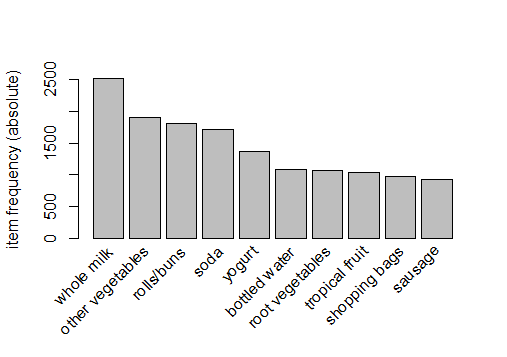
\includegraphics[scale=0.60]{img1.png}}
		\label{fig:usecase}
	\end{figure}
\end{center}  
			
\newpage
\section{CONCLUSION : }
Hence, we have  Build a required Database to develop BAI tool for considering one aspect of growth to the business Such as organization of products based on demand and patterns use R Programming.

\end{document}